\begin{figure}[p]
\centering
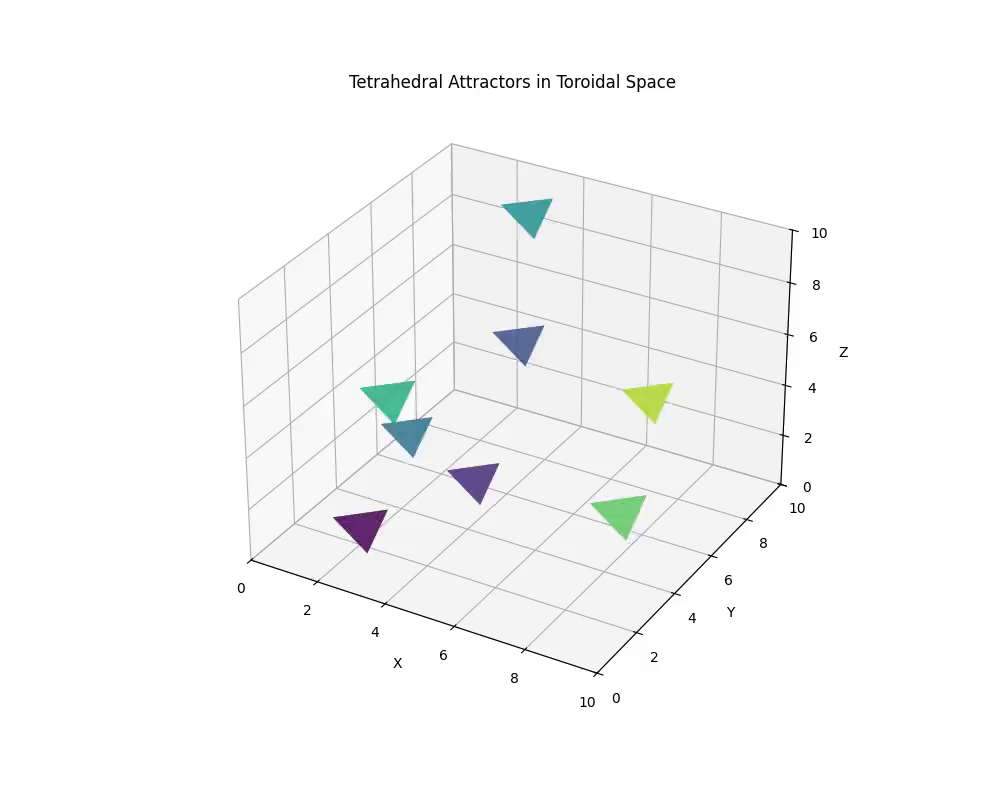
\includegraphics[width=0.485\linewidth,height=0.32\textheight,keepaspectratio]{figures/F06_0.png}
\hfill
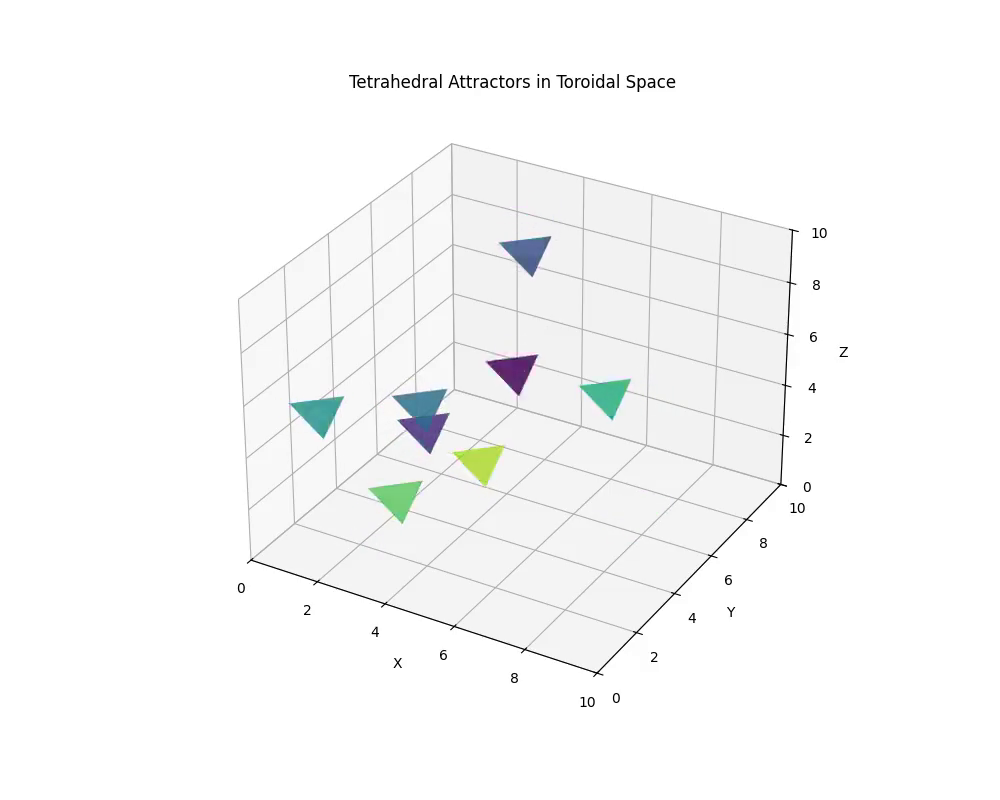
\includegraphics[width=0.485\linewidth,height=0.32\textheight,keepaspectratio]{figures/F06_1.png}
\par\medskip
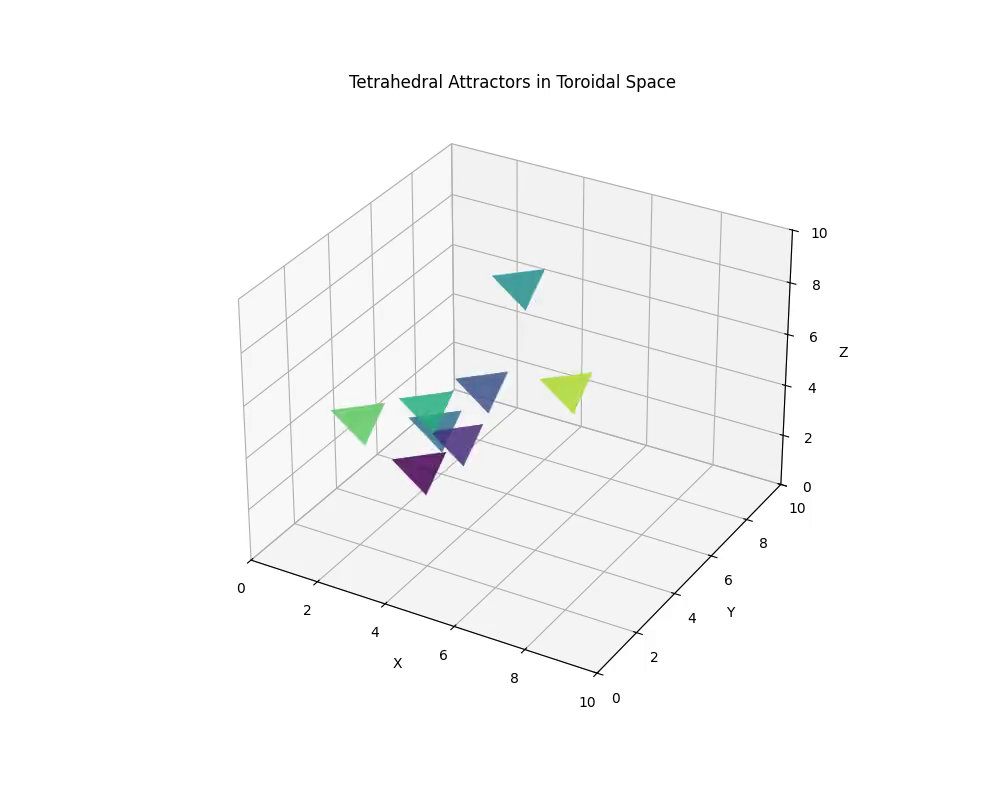
\includegraphics[width=0.485\linewidth,height=0.32\textheight,keepaspectratio]{figures/F06_2.png}
\hfill
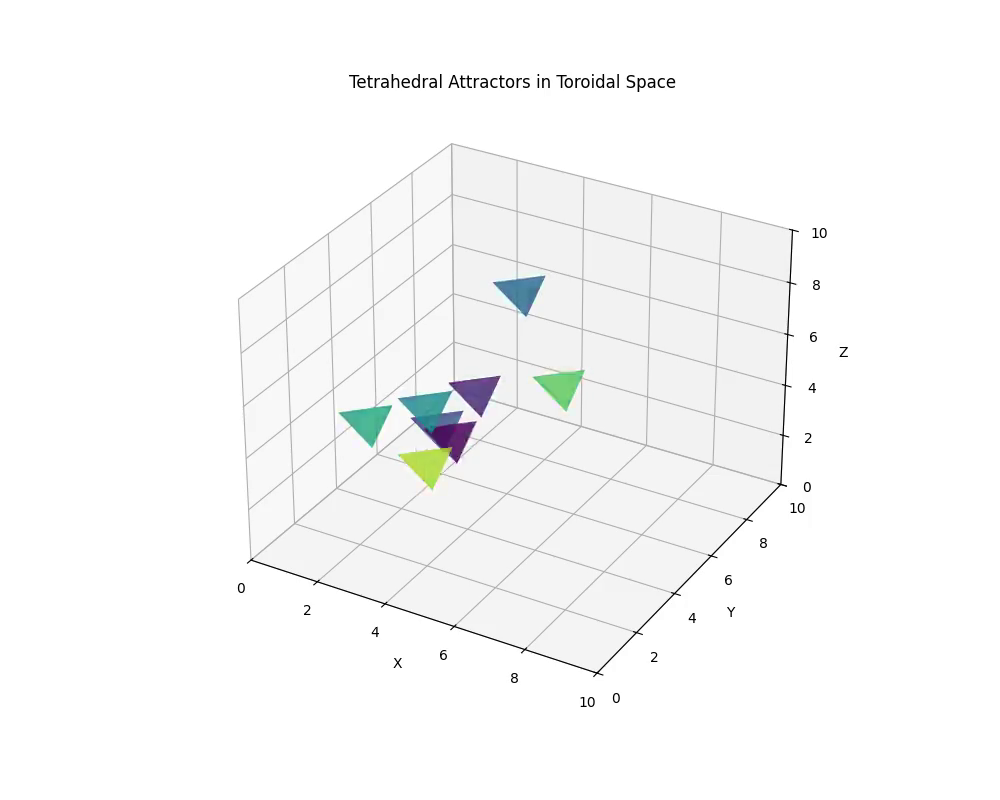
\includegraphics[width=0.485\linewidth,height=0.32\textheight,keepaspectratio]{figures/F06_3.png}
\par\medskip
\caption[Four stages of the source-associated S02 movie]{ORIGINAL movie content / ATTRIBUTED, decoded stills. S02 frames 0,30,600,1999 in reading order (0,0.5,10,33.3167 movie seconds). The XYZ axes cover 0--10 in source coordinates. Projection shows changing arrangements and smaller late screen motion, not measured 3D speeds or convergence. Decoded in the accepted Construction 02 study; no new state was generated. \cite{construction02}}
\label{fig:F06}
\end{figure}
